\documentclass[11pt]{article}
\usepackage[top=1in, bottom=1in, left=1in, right=1in]{geometry}

\usepackage{amsmath}
\usepackage{amssymb}
\usepackage{graphicx}

\title{Quiz \#0 (Diagnostic Quiz), 8/23 \\ Math 156 (Calculus I), Fall 2022}
\date{}

\begin{document}

\maketitle

\thispagestyle{empty}

\vspace{-1cm}

This quiz is designed to check your background in high school algebra. It will not be graded.

\begin{enumerate}
\item Simplify the following expressions:
\[ \mathrm{(a)} \; \; (-3)^4 \qquad \mathrm{(b)} \; \; 3^{-4} \qquad \mathrm{(c)} \; \; \frac{5^{23}}{5^{21}} \qquad \mathrm{(d)} \; \; \sqrt{200}-\sqrt{32} \qquad \mathrm{(e)} \; \; (3a^3b^3)(4ab^2)^2 \]
\item Solve the following equations:
\[ \mathrm{(a)} \; \; \frac{2x}{x+1} = \frac{2x-1}{x} \qquad \mathrm{(b)} \; \; x^2 - x -12 = 0\]
\item Decide whether each of these identities is true or false:
\[ \mathrm{(a)} \; \; (p+q)^2 = p^2 + q^2 \qquad \mathrm{(b)} \; \; \sqrt{ab} = \sqrt{a}\sqrt{b}  \]
\item Find the equation of a line that passes through point $(2,-5)$ and is parallel to line $2x-4y=3$.

\item Consider the function $f$ graphed below:
\[ 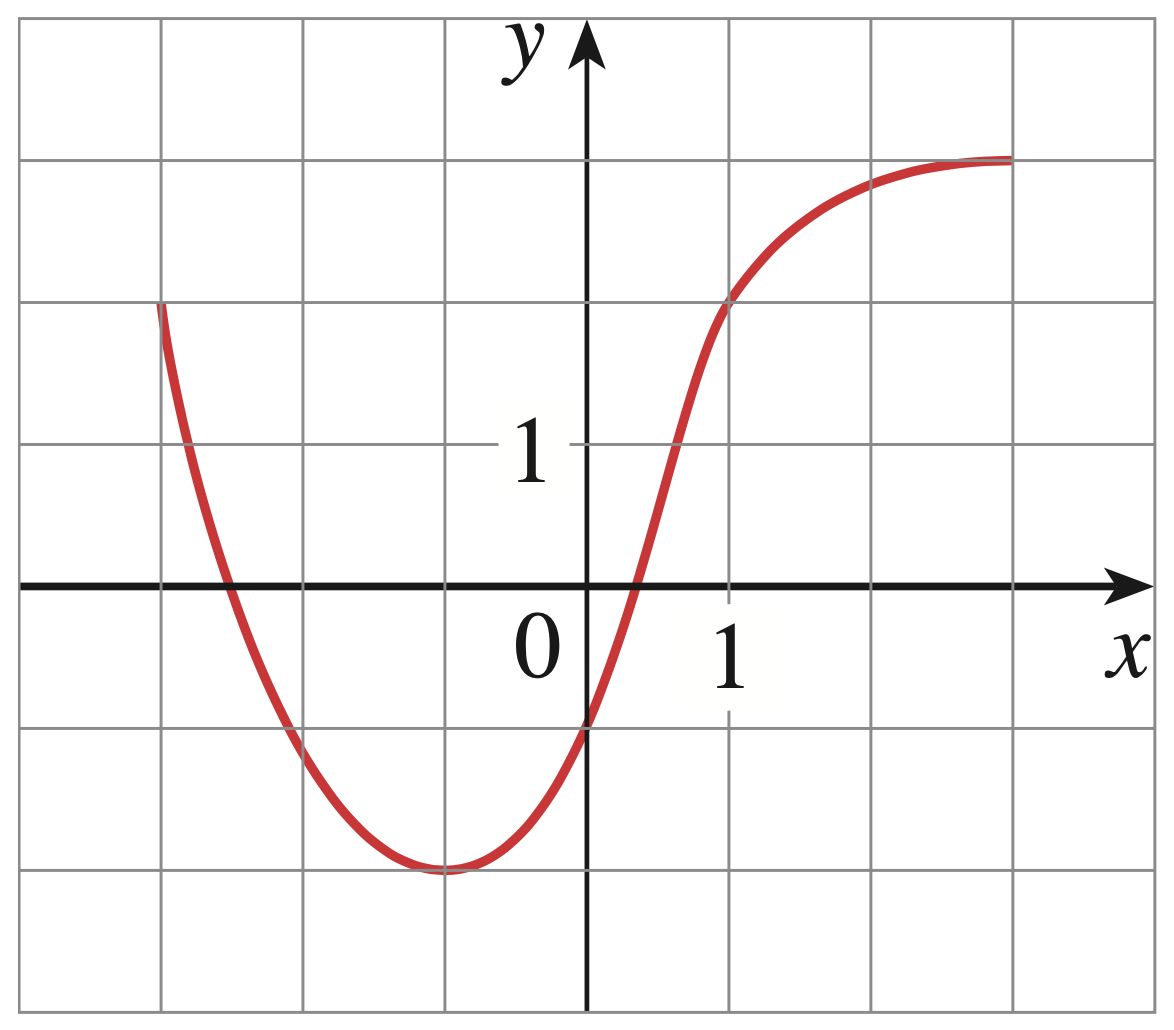
\includegraphics[width=2in]{quiz_0_fn.png} \]
\begin{enumerate}
\item State the value of $f(-1)$.
\item Estimate the values of $x$ for which $f(x)=0$.
\item What are the domain and the range of $f$?
\end{enumerate}

\item Convert from degrees to radians (for (a) and (b)) or radians to degrees (for (c)):
\[ \mathrm{(a)} \; \; 300^{\circ} \qquad \mathrm{(b)} \; \; -18^{\circ} \qquad \mathrm{(c)} \; \; \frac{5\pi}{6}\]

\item Find the exact value of these evaluations of trigonometric functions (assume input is radians):
\[ \mathrm{(a)} \; \; \tan(\pi/3) \qquad \mathrm{(b)} \; \; \sin(7\pi/6)\]

\end{enumerate}

\end{document}
